% Options for packages loaded elsewhere
\PassOptionsToPackage{unicode}{hyperref}
\PassOptionsToPackage{hyphens}{url}
%
\documentclass[
]{book}
\title{Nature hacks for life}
\author{cjlortie}
\date{}

\usepackage{amsmath,amssymb}
\usepackage{lmodern}
\usepackage{iftex}
\ifPDFTeX
  \usepackage[T1]{fontenc}
  \usepackage[utf8]{inputenc}
  \usepackage{textcomp} % provide euro and other symbols
\else % if luatex or xetex
  \usepackage{unicode-math}
  \defaultfontfeatures{Scale=MatchLowercase}
  \defaultfontfeatures[\rmfamily]{Ligatures=TeX,Scale=1}
\fi
% Use upquote if available, for straight quotes in verbatim environments
\IfFileExists{upquote.sty}{\usepackage{upquote}}{}
\IfFileExists{microtype.sty}{% use microtype if available
  \usepackage[]{microtype}
  \UseMicrotypeSet[protrusion]{basicmath} % disable protrusion for tt fonts
}{}
\makeatletter
\@ifundefined{KOMAClassName}{% if non-KOMA class
  \IfFileExists{parskip.sty}{%
    \usepackage{parskip}
  }{% else
    \setlength{\parindent}{0pt}
    \setlength{\parskip}{6pt plus 2pt minus 1pt}}
}{% if KOMA class
  \KOMAoptions{parskip=half}}
\makeatother
\usepackage{xcolor}
\IfFileExists{xurl.sty}{\usepackage{xurl}}{} % add URL line breaks if available
\IfFileExists{bookmark.sty}{\usepackage{bookmark}}{\usepackage{hyperref}}
\hypersetup{
  pdftitle={Nature hacks for life},
  pdfauthor={cjlortie},
  hidelinks,
  pdfcreator={LaTeX via pandoc}}
\urlstyle{same} % disable monospaced font for URLs
\usepackage{longtable,booktabs,array}
\usepackage{calc} % for calculating minipage widths
% Correct order of tables after \paragraph or \subparagraph
\usepackage{etoolbox}
\makeatletter
\patchcmd\longtable{\par}{\if@noskipsec\mbox{}\fi\par}{}{}
\makeatother
% Allow footnotes in longtable head/foot
\IfFileExists{footnotehyper.sty}{\usepackage{footnotehyper}}{\usepackage{footnote}}
\makesavenoteenv{longtable}
\usepackage{graphicx}
\makeatletter
\def\maxwidth{\ifdim\Gin@nat@width>\linewidth\linewidth\else\Gin@nat@width\fi}
\def\maxheight{\ifdim\Gin@nat@height>\textheight\textheight\else\Gin@nat@height\fi}
\makeatother
% Scale images if necessary, so that they will not overflow the page
% margins by default, and it is still possible to overwrite the defaults
% using explicit options in \includegraphics[width, height, ...]{}
\setkeys{Gin}{width=\maxwidth,height=\maxheight,keepaspectratio}
% Set default figure placement to htbp
\makeatletter
\def\fps@figure{htbp}
\makeatother
\setlength{\emergencystretch}{3em} % prevent overfull lines
\providecommand{\tightlist}{%
  \setlength{\itemsep}{0pt}\setlength{\parskip}{0pt}}
\setcounter{secnumdepth}{5}
\usepackage{booktabs}
\ifLuaTeX
  \usepackage{selnolig}  % disable illegal ligatures
\fi
\usepackage[]{natbib}
\bibliographystyle{apalike}

\begin{document}
\maketitle

{
\setcounter{tocdepth}{1}
\tableofcontents
}
\hypertarget{sustainability}{%
\chapter{Sustainability}\label{sustainability}}


\includegraphics[width=4in,height=\textheight]{./tree.png}\\
This is the prework before we meet.

\hypertarget{context}{%
\subsection*{Context}\label{context}}
\addcontentsline{toc}{subsection}{Context}

Nature deficit disorder

Reciprocal restoration

Sustainability and feedback loops

\hypertarget{learning-outcomes}{%
\subsection*{Learning outcomes}\label{learning-outcomes}}
\addcontentsline{toc}{subsection}{Learning outcomes}

\begin{enumerate}
\def\labelenumi{\arabic{enumi}.}
\tightlist
\item
  Build a tidy, logical data model for a graduate-level dataset.\\
\item
  Develop a reproducible data and statistical workflow.\\
\item
  Design and complete intermediate-level data visualizations appropriate for a graduate-level tidy dataset.\\
\item
  Identify a range of suitable univariate or multivariate statistical approaches that can be applied to any dataset.\\
\item
  Interpret statistical output to quantify statistical model performance.\\
\item
  Complete fundamental exploratory data analysis on a representative dataset.\\
\item
  Appreciate the strengths and limitations of open science, data science, and evidence-based collaboration models.
\end{enumerate}

\hypertarget{schedule}{%
\subsection*{Schedule}\label{schedule}}
\addcontentsline{toc}{subsection}{Schedule}

Slide decks are optional. The decks simply highlight some of the connections between the criteria for critical thinking and statistical heuristics.

\begin{tabular}{rll}
\toprule
week & challenge & tasks\\
\midrule
1 & Explore sustainability and reciprocity with natural systems & take ecological footprint quiz, track simple life decisions, list frictions and resistance\\
2 & Nature hacks deck and discussion & reflect on meaning, list purpose, match challenges with nature\\
3 & Practice & explore nature practice, track creativity, track breath\\
4 & Next steps & futureproof daily practice, identify resolutions that are more significant challenges\\
\bottomrule
\end{tabular}

\hypertarget{citation}{%
\subsection*{Citation}\label{citation}}
\addcontentsline{toc}{subsection}{Citation}

Lortie, CJ (2021): A primer for biostatistics in R. figshare. Book. \url{https://doi.org/10.6084/m9.figshare.15048597.v2}

\hypertarget{license}{%
\subsection*{License}\label{license}}
\addcontentsline{toc}{subsection}{License}

This work is licensed under a Creative Commons Attribution-NonCommercial-ShareAlike 4.0 International License.

\hypertarget{challenge-time}{%
\subsection*{Challenge time}\label{challenge-time}}
\addcontentsline{toc}{subsection}{Challenge time}

Do the footprint quiz.

\hypertarget{reflection-questions}{%
\subsection*{Reflection questions}\label{reflection-questions}}
\addcontentsline{toc}{subsection}{Reflection questions}

\begin{enumerate}
\def\labelenumi{\arabic{enumi}.}
\tightlist
\item
  What can a t-test do? Can you imagine other functions for a t-test in the context of your work and life?
\item
  What are the limitations of a t-test?
\item
  Is the data structure wide, long, and how can you consider tidying this evidence? Are there variables that represent the same concept?
\end{enumerate}

\hypertarget{hacks}{%
\chapter{Nature hacks}\label{hacks}}

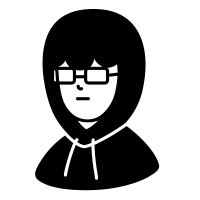
\includegraphics[width=3in,height=\textheight]{./hacker.png}

Many approaches and critical thinking heuristics in ecology \& evolutionary biology (eeb) are relevant to other disciplines.

\hypertarget{context-1}{%
\subsection*{Context}\label{context-1}}
\addcontentsline{toc}{subsection}{Context}

\hypertarget{learning-outcomes-1}{%
\subsection*{Learning outcomes}\label{learning-outcomes-1}}
\addcontentsline{toc}{subsection}{Learning outcomes}

\begin{enumerate}
\def\labelenumi{\arabic{enumi}.}
\tightlist
\item
  Develop your data viz skills.\\
\item
  Hone your critical thinking statistically by iterative plotting-modeling a dataset.\\
\item
  Do a regression analysis.
\end{enumerate}

\hypertarget{challenge-time-1}{%
\subsection*{Challenge time}\label{challenge-time-1}}
\addcontentsline{toc}{subsection}{Challenge time}

\hypertarget{reflection-questions-1}{%
\subsection*{Reflection questions}\label{reflection-questions-1}}
\addcontentsline{toc}{subsection}{Reflection questions}

\begin{enumerate}
\def\labelenumi{\arabic{enumi}.}
\tightlist
\item
  When do you use regression versus correlation?\\
\item
  How could you incorporate time into your plots or statistical models?\\
\item
  Did the visualization highlight some of the criteria associated with critical thinking statistically more than others?
\end{enumerate}

\hypertarget{practice}{%
\chapter{Daily practice}\label{practice}}

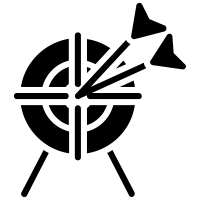
\includegraphics[width=3in,height=\textheight]{./practice.png}

\hypertarget{context-2}{%
\subsection*{Context}\label{context-2}}
\addcontentsline{toc}{subsection}{Context}

Exploratory data analyses is everything we have done. This is a primary approach to better understanding your evidence without introducing bias. Transparency is key.

\hypertarget{learning-outcomes-2}{%
\subsection*{Learning outcomes}\label{learning-outcomes-2}}
\addcontentsline{toc}{subsection}{Learning outcomes}

\begin{enumerate}
\def\labelenumi{\arabic{enumi}.}
\tightlist
\item
  Practice your critical workflow for data and statistics that is replicable and literate.\\
\item
  Appreciate the value of generalized statistical models that connect to one another conceptually.\\
\item
  Do a GLM.
\end{enumerate}

\hypertarget{challenge-time-2}{%
\subsection*{Challenge time}\label{challenge-time-2}}
\addcontentsline{toc}{subsection}{Challenge time}

Here is an impressive ..

\hypertarget{reflection-questions-2}{%
\subsection*{Reflection questions}\label{reflection-questions-2}}
\addcontentsline{toc}{subsection}{Reflection questions}

\begin{enumerate}
\def\labelenumi{\arabic{enumi}.}
\tightlist
\item
  When do you move from EDA to model fitting?\\
\item
  Are there ways to mitigate bias and \href{https://www.wired.com/story/were-all-p-hacking-now/}{p-hacking} through formal workflows?\\
\item
  Did building a model such as GLM align with critical thinking and intuition, i.e from critical thinking was it accurate and fair? Did the EDA-to-model process legitimately represent the patterns in the observations recorded.
\end{enumerate}

\hypertarget{consolidate}{%
\chapter{Consolidate}\label{consolidate}}

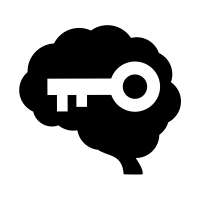
\includegraphics[width=3in,height=\textheight]{./brain.png}

\hypertarget{context-3}{%
\subsection*{Context}\label{context-3}}
\addcontentsline{toc}{subsection}{Context}

\hypertarget{learning-outcomes-3}{%
\subsection*{Learning outcomes}\label{learning-outcomes-3}}
\addcontentsline{toc}{subsection}{Learning outcomes}

\begin{enumerate}
\def\labelenumi{\arabic{enumi}.}
\tightlist
\item
  Practice your critical workflow for data and statistics that is replicable and literate.\\
\item
  Appreciate the value of generalized statistical models that connect to one another conceptually.\\
\item
  Do a GLM.
\end{enumerate}

\hypertarget{challenge-time-3}{%
\subsection*{Challenge time}\label{challenge-time-3}}
\addcontentsline{toc}{subsection}{Challenge time}

Here is an impressive

\hypertarget{reflection-questions-3}{%
\subsection*{Reflection questions}\label{reflection-questions-3}}
\addcontentsline{toc}{subsection}{Reflection questions}

\begin{enumerate}
\def\labelenumi{\arabic{enumi}.}
\tightlist
\item
  When do you move from EDA to model fitting?\\
\item
  Are there ways to mitigate bias and \href{https://www.wired.com/story/were-all-p-hacking-now/}{p-hacking} through formal workflows?\\
\item
  Did building a model such as GLM align with critical thinking and intuition, i.e from critical thinking was it accurate and fair? Did the EDA-to-model process legitimately represent the patterns in the observations recorded.
\end{enumerate}

  \bibliography{book.bib,packages.bib}

\end{document}
